\documentclass[journal]{IEEEtran}

\usepackage{cite}
\usepackage{graphicx}
\usepackage{amsmath}
\usepackage{algorithmic}

\begin{document}
\title{Political Districting via Discrete Particle Swarm Optimization}
\author{~David~Fu,~David~Zhang,~Ellen~Wang,~Leslie~Reyes,~Seikun~Kambashi,~Shiranka~Miskin}
\maketitle

\begin{abstract}
% The Summary should be a brief version of the full report. It should give the
% reader an accurate overview. Be brief, but be specific.
% reader an accurate overview. Be brief, but be specific.
Political Districting is a crucial aspect of the American political system which
    causes much controversy as groups attempt to divide states in ways that
    benefit specific agendas.  The particle swarm optimization method proposed
    in this paper attempts to generate fair and bipartisan districting
    solutions, optimizing for population equality and district compactness.  The
    effectiveness of the particle swarm method was then compared with Simulated
    Annealing, Tabu search, and Hill Climbing.  Evaluations were performed on
    faked sample data, as well as data on the state of Iowa using 2016 census
    data.  The particle swarm method was outperformed only by tabu search, and
    further investigation into this method is recommended.
\end{abstract}

\section{Introduction}
% Summarize the importance of the problem you are trying to solve and the reason
% that motivated you to select this project. Explain what was the problem or
% challenge that you were given? state the purpose of the project and how did
% you solve it? Enumerate the objectives of the project and describe in brief
% the structure of the report.
\subsection{Problem Importance}
Political districting\cite{redistricting} is a process where geographic territories must be
subdivided into electoral districts. This process is significant to democracies,
since a district elects a single member to the parliament. It is essential
maintain fairness, and that the overall arrangement of electoral districts are
not designed to be advantageous to any particular political party.

The process of political districting is usually carried through by a neutral
party that attempts to satisfy legislative criteria\cite{legislature}. However, criteria used
to generate district boundaries can be heavily disputed, and it is easy to
introduce bias through manual intervention. Gerrymandering is an effect that
occurs when boundaries are generated in a way that exploits voting patterns
of the population in attempt to favour some political parties over others\cite{gerry}.
One symptom of Gerrymandering is the creation of skewed, irregularly concave
electoral district boundaries.

In interest of political neutrality and fairness, it is important to avoid
suspicion of interference and  Gerrymandering. Use of mathematical models
and search algorithms have been explored to subdivide territory into fair
electoral district boundaries. Some of the most commonly accepted criteria
include the contiguity of districts, population equity, and geographic
compactness of district boundaries. Although the weights of the algorithm
require manual input, they could ideally be adjusted to satisfy different
parties of interest.

We chose to tackle to problem of political districting because exploring
solutions could have implications on society. We found this area of work
to be very motivating to work on and more relevant to us than some of the
other projects. In addition to tackling interesting problems in AI, it would
also educate us about how some of the political systems of our world work,
and where they have drawbacks.


\subsection{Project}
The problem we were presented was as follows: given a geographic territory
with data describing how its population is distributed, subdivide the
population into m contiguous districts. Solutions are most preferable
when the districts contain near-equal populations and are geographically compact.

The purpose of the project is to explore which algorithm implementations
would produce solutions that were most preferable for our smaller, simplified
data sets. We would do this by working with smaller, controlled data sets on
geographic population and implementing multiple algorithms to assess their
relative performance.

Specifically, we investigated the relative performance of Tabu search,
TSP-based and geometric semantic genetic algorithms, and mini-max spanning
forest algorithm implementations. These algorithms were run on data both
hand-made and retrieved from US census data on state population distributions.
The effectiveness of each algorithm was assessed using a fitness criteria that
we created, which assesses the population equity, contiguity, and compactness
of all districts generated by an instance of the algorithms.

\subsection{Report Structure}
This report will first review some of the existing papers on solving the
political districting problem using local search methods. A number of
papers were consulted for algorithm implementation, which assisted us
in programming our implementations of particle swarm optimization, simulated
annealing, and Tabu search algorithms. We will discuss how the papers were
used and what extensions were made to our findings.

Next, the report will formally define the political districting problem using
problem formulation. The report will discuss the data taken from the US Census
and our solution processes this data to setup the problem.

Finally, we will discuss the solution we chose to approach the political
districting problem and evaluate its performance and effectiveness. We will
also analyze the results and compare them to findings in literature, arriving
at our own conclusions about how our solution can be used to solve political
districting.

\section{Literature Review}
% Conduct a critical survey on similar solutions and explain how your solution
% extends or differs from these solutions.
\subsection{Particle Swarm Optimization}
The paper Particle Swarm Optimization for Travelling Salesman Problem\cite{tsp-pso}
discusses how the particle swarm optimization (PSO) method can be used to
solve TSP-based problems. Although redistricting tackles a conceptually
different problem than TSP, the paper’s approach of using swap operators
and sequences allowed us to implement our PSO algorithm on top of the
redistricting problem.

\subsection{Tabu Search}
In A Tabu Search Heuristic and Adaptive Memory Procedure for Political
Districting\cite{local-search}, the authors uses Tabu search to tackle the problem of
political redistricting. They define successful solution using the standard
criteria, i.e. population equity, district contiguity, and district compactness.

The paper gave valuable insight on how to design initial solutions and
Tabu tenure for our implementation. Additionally, the approaches used to
calculate population equality and compactness as per our fitness criteria
were borrowed directly from the equations provided in the paper. Direct
implementation of Tabu search from findings in this paper allowed us to
compare results from our PSO solution to other types of local search.

\section{Problem Formulation and Modeling}
% Include the problem statement and describe its model.
The Political Districting problem can be modeled as an assignment problem with
specific constraints.  The goal is to assign a fixed set of tracts to a fixed
number of districts, where each district is contiguous, while minimizing a
certain cost function.  The inputs provided to our algorithms are:

\begin{itemize}
\item $T$, The set of tracts
\item $D$, the set of Districts
\item $P_T(x)$ which gives the population of a given tract
\item $A_T(x)$ which gives the area of a given tract
\item $Borders(x)$ which, for a given tract, returns the set of tracks adjacent to it paired with the lengths of those borders
\end{itemize}

We define a solution as a mapping $s: T \rightarrow D$ where every unit in $T$
is mapped to a single district in $D$, and every district in $D$ has at least
one unit in $T$ assigned to it.  The encoding method does not make any effort to
guarantee district contiguity, therefore it is left to the algorithm to only
generate valid solutions.

\section{Proposed Solution}
\label{sec:proposed_solution}
Particle Swarm Optimization is an optimization technique which models particles
moving through a continuous n-dimensional search space, where each particle
represents a potential solution to the problem.  In the classical PSO algorithm,
a set of particles are initialized to a certain solution, then at each
iteration, each particle computes its next position via the following equations
of motion:

\begin{equation}
\label{vel-update-eqn-classic}
\begin{aligned}
v_{t + 1}^{id} &= w \cdot v_t^{id}\\
&+ c_1r_1^{id}(lbest_t^{id} - x_t^{id})\\
&+ c_2r_2^{id}(gbest_t^{id} - x_t^{id})\\
\end{aligned}
\end{equation}
\begin{equation}
\label{pos-update-eqn-classic}
x_{t + 1}^{id} = x_t^{id} + v_{t + 1}^{id}
\end{equation}

Where $v$ is the velocity of particle $id$, $w$ is the inertia weight, $c_1,
c_2$ are acceleration coefficients, $r_1, r_2$ are randomly generated numbers in
$[0, 1]$, $x$ is the position of the particle, $lbest$ is the best solution the
particle has traversed, $gbest$ is the best solution traversed across all
particles, $t$ is the iteration number, and $i$ and $d$ are the particle number
and dimension.  While this algorithm was meant for problems on a continuous
space, it can also be used for discrete optimization problems.  Our solution,
inspired by the work of Kang-Ping Wang et al. \cite{tsp-pso} on the Traveling
Salesman Problem, proposes a novel method of applying PSO to the discrete
problem of Political Districting.

\subsection{Initial Solution}
% Generate an initial solution.
In order to generate a valid initial solution, we proceed as in Vickrey
\cite{initial} and Bozkaya \cite{local-search}.  Initially, all tracts are not
yet assigned to any district. The goal of this algorithm is to generate an
initial solution such that all tracts are assigned to exactly $|D|$ contiguous
districts.

For the purpose of this algorithm, we define a target population for the
districts in the initial solution:
$$\bar{P} = \frac{\sum_{x \in T} P_T(x)}{|D|}$$

We create our districts by picking an unassigned seed tract, and then gradually
add randomly picked unassigned adjacent tracts to the district until the
population of the district exceeds $\bar{P}$ for the first time, or there are no
unassigned adjacent tracts available. We do this until all the tracts are
assigned to a district.

The result of this initial assignment could result in $k$ districts that may or
may not be equal to $|D|$.

If $k > |D|$, we iteratively pick the district with the smallest population, and
merge it with its smallest neighbour to preserve contiguity. In the case where
$k < |D|$, we iteratively increase the number of districts by splitting the
district with the largest population into two districts while still preserving
contiguity. At the end of this process, there will be exactly $|D|$ valid
districts that can be used as an initial solution.

\subsection{Cost Function}
% Suggest a cost function (objective function) suitable for this problem.
While there are many factors that can be considered for political districting,
for the sake of efficiency and simplicity, our fitness function only focuses on
the two main goals of political districting which are population equality and
district compactness.  These measures do not assess the contiguity of a
solution, as the algorithms used are designed to only evaluate valid solutions.
A constant coefficient is introduced to each term to allow us to tune how much
each factor contributes to the overall fitness.

$$f(x) = c_{pop} \cdot f_{pop}(x) + c_{shape} \cdot f_{shape}(x)$$

\subsubsection{Population Equality}
In an ideal solution, each district would have the same population, which would
equal the average population across the districts.  We therefore define the
measure of population equality for a set of districts $D$ where $P_D(d)$ is the
total population of district $d \in D$ as
$$f_{pop}(x) = \sum_{d \in D} P_D(d) - \bar{P}$$

\subsubsection{Compactness}
To evaluate compactness we use the Schwartzberg Index\cite{schwartzberg}, which
is the perimeter of a district squared divided by its area, due to it being
simple to compute.  The perimeter of a district is computed by summing up the
outward border lengths of the tracts on its border, and the area of a district
is computed as the sum of the tract areas.

$$f_{shape} = \sum_{d \in D} \frac{(P_D(d))^2}{A_D(d)}$$

\subsection{Neighborhood}
% Define a suitable neighborhood operator.
The neighborhood of a given solution is defined as all possible solutions
reachable by moving one tract from district $i$ to district $j$ such that the
resulting solution remains contiguous.


\subsection{Algorithm Description}
% Define a suitable solving strategy for this problem.
In order to apply Particle Swarm Optimization on our problem we must define
sufficient terminology and mathematical operators to be able to perform the
update function \ref{vel-update-eqn-classic}.\\

\subsubsection{Velocity}
For the discrete solution space of district assignment, we define "velocity" to
be an ordered sequence of Swap Operators.  A given Swap Operator $SO(t, d)$ is
defined as taking tract $t$ belonging to district $d_o$ and being reassigned to
district $d$, where $d_o \neq d$.\\

\subsubsection{Initial Velocity and Inertia}
Initial particle velocities are generated by performing random swaps that still
generate valid solutions.  The $v$ term in \ref{vel-update-eqn-classic} is also
generated as a random sequence of swaps, where the length of this sequence is a
constant parameter.  As a result, the concept of "inertia" is not present in our
solution.\\

\subsubsection{Addition of Velocity to a Solution}
Given a solution $X$ and a velocity $V = (SO_1, SO_2, \cdots SO_m)$, $X + V$ is
the solution resulting from the application of swaps $SO_1 \cdots SO_m$ on $X$
in ascending order.  In order to assure that the algorithm only produces valid
solutions, the resulting state must be contiguous.\\

\subsubsection{Subtraction of Solutions from Solutions}
Given two valid solutions $A$ and $B$, the subtraction operator $A - B = V$ is a
velocity described as a sequence of swaps required to transform solution $B$
into $A$.  The resulting velocity $V$ is guaranteed to be valid when applied to
solution $A$, as $B$ is assumed to be valid.  In our implementation, this
sequence is determined by iterating through districts in $B$ and applying $SO(t,
d)$ if tract $t$ is assigned to district $d$ in solution $A$ but not in solution
$B$, and the result remains contiguous.\\

\subsubsection{Multiplication of Real Numbers and Velocities}
Given $V = (SO_1, \cdots SO_m)$ we define $c \cdot V, c \in [0, 1]$ as the
sequence constructed from the first $\lceil c\cdot m \rceil$ swap operators in
$V$.  Any values of $c$ outside of $[0, 1]$ are considered invalid.\\

\subsubsection{Modified Update}
To perform equation~\ref{pos-update-eqn-classic}, changes must be made
to~\ref{vel-update-eqn-classic} to guarantee that $x_{t}^{id} + v_{t + 1}^{id}$
results in a contiguous solution. Naively
performing~\ref{vel-update-eqn-classic} would result in the $w \cdot v_t^{id}$,
$c_1r_1^{id}(lbest_t^{id} - x_t^{id})$, and $c_2r_2^{id}(gbest_t^{id} -
x_t^{id})$ being valid on $x_t^{id}$, however in order to add these resulting
velocities to calculate $v_{t + 1}^{id}$, we cannot simply append the swap
sequences.  Even if swap sequences $v_1$ and $v_2$ are both valid on solution
$x$, $v_2$ is not guaranteed to be valid on $x + v_1$.  We therefore use a
modified position update method
\begin{equation}
\begin{aligned}
X_1 &= x_{t}^{id} + w \cdot v_{t}^{id}\\
X_2 &= X1 + r_1 \cdot c_1 \cdot (lbest_{t}^{id} - X_1)\\
x_{t + 1}^{id} &= X_2 + r_2 \cdot c_2 \cdot (gbest_t^{id} - X_2)\\
\end{aligned}
\end{equation}

Since the $r_1 \cdot c_1 \cdot (lbest_{t}^{id} - X_1)$ term of $X_2$ is
generated from $X_1$, adding the first $i$ elements of that result to $X_1$ is
guaranteed to be a contiguous solution.  The same reasoning can be applied to
conclude that $x_{t + 1}^{id}$ is a valid solution\\

This method of addition differs from the classical vector addition, however it
achieves the same goal of having a particle move in the direction of a velocity,
in the direction of the local best, and in the direction of the global best,
each to some variable degree.  One important difference to note, is that if each
coefficient was $1$, even though each velocity is applied "equally", $X_2$ would
be equivalent to $lbest$, and $x_{t + 1}$ would be equivalent to $gbest$.  This
detail can be handled by tuning the constant terms.\\

\subsubsection{Implementation Details}
The computation of $A - B$ where $A$ and $B$ are solutions is expensive, as the
process of getting from $A$ to $B$ may require a very large number of swaps.  We
therefore introduce a constant parameter which describes the maximum number of
swaps to generate when calculating $A - B$.  Another issue with a naive
implementation is that when generating a random velocity, certain swaps may undo
previous swaps.  To avoid this, a tabu list is maintained, which disallows
assigning a cell to a district it had previously been assigned to during that
swap sequence.\\


\subsubsection{Possible Improvements}
There are certain ideas which we did not have time to implement, however may
theoretically result in improvements in performance and solution quality.  While
our current implementation has no concept of "inertia", we could define
"inertia" to be related to which districts grew or shrunk during the previous
iteration.  To create the swap sequence $v_{t} = SO_{t, 1} .. SO_{t, m}$ that is
valid on $x_t$, and inherits the inertia of $v_{t - 1} = SO_{t - 1, 1} .. SO_{t
- 1, m}$, we would ensure that for $SO_{t - 1, i} = (u_{t - 1}, d_{t - 1}$ and
$SO_{t, i} = (u_t, d_t)$, $d_{t - 1} = d_t$ and $s(u_{t - 1}) = s(u_t)$.  This
means that every swap in each swap sequence will take a tract from district $i$
and move it to district $j$, the only difference between the sequences is which
tract was swapped.  Another possible improvement would be to establish certain
"centers" for each district, similar to what was done in the work by Federica
Ricca et al.\cite{voronoi}.  Each district would have one "center" tract which
is always assigned to that district.  This means that between two solutions,
each district $d$ will be in the same general area.  This trait would
theoretically help the efficiency of the algorithm immensely, as in the current
implementation, two equivalent districting solutions could be seen as radically
different simply because the specific identifiers assigned to the districts are
different.


\subsection{Parameter Values}
% Select your own values for the parameter and explain the basis for your selection.
We tested arbitrary combinations of values for $w$, $c_1$, and $c_2$ where $w, c_1, c_2 <= 1$ because of the constraints set by how we defined a particle's velocity. A parameter value greater than $1$ would not have made any sense given our velocity model. The swarm size was limited by our computing power to 5 particles.

\subsection{Example Run-through}
% Describe how each algorithm (TS, SA, GA, PSO and ACO) will proceed to solve
% this problem by performing at least two hand iterations on a reduced version
% of the problem.
We will demonstrate two iterations of the three algorithms we have chosen to implement using a simple example input.
The input's tracts are conceptually a grid of tracts, where each tract shares a border with its vertical and horizontal neighboring tracts.

The population of each tract is 1 for simplicity, and the solution will be a grouping of tracts such that there are exactly two groups that represent two districts. \\

\subsubsection{Simulated Annealing}~\\
\begin{figure}[h!]
    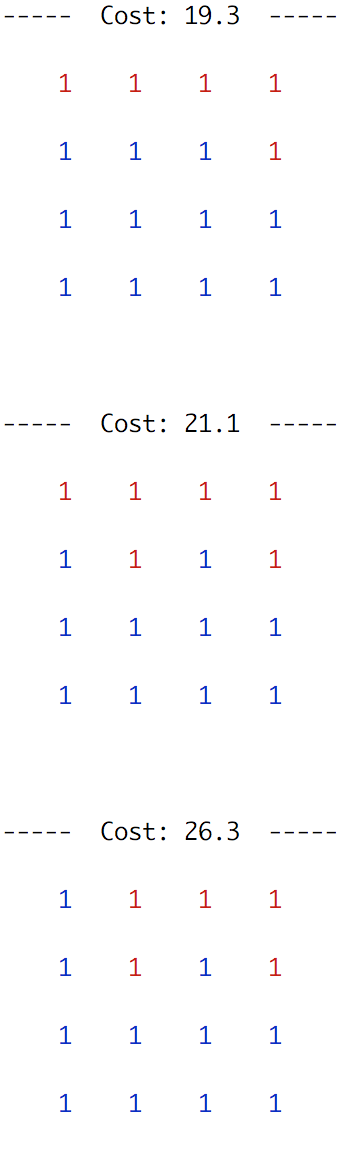
\includegraphics[width=3cm]{sa.png}
    \centering
    \caption{Example run using Simulated Annealing}
        \label{fig:sa_example}
\end{figure}

Figure \ref{fig:sa_example} shows the first two iterations of the SA implementation.
We start with a randomly generated initial solution of two districts with a fitness cost of 19.3 (calculated using the previously defined cost function).

The neighborhood of the initial solution is defined by the set of possible tract swaps (switching a tract from one district to another) without breaking continuity.

The algorithm will randomly pick one of these neighbors, and will choose it as the new solution if its fitness is better than the current one, or if the acceptance probability given the current temperature allows for worser solutions.

The algorithm does not stop in the first two iterations since the stopping conditions have not been met. Since the temperature is quite high in the beginning, the first two iterations also end up accepting solutions that have a worse fitness than the previous solution. \\

\subsubsection{Tabu Search}~\\
\begin{figure}[h!]
    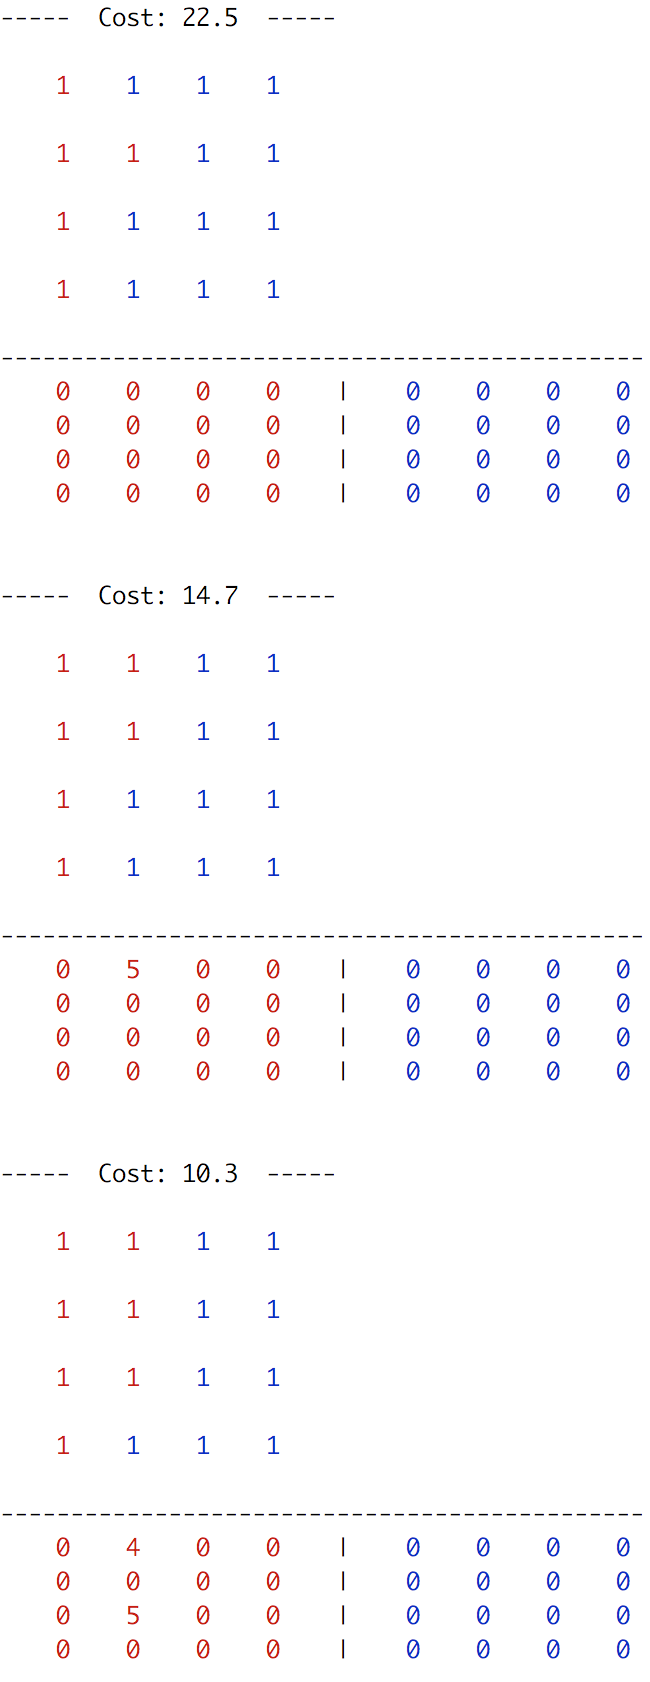
\includegraphics[width=6cm]{tabu.png}
    \centering
    \caption{Example run using Tabu Search}
        \label{fig:tabu_example}
\end{figure}
Figure \ref{fig:tabu_example} shows the first three iterations of a sample run using our tabu search implementation. Similarly to our SA algorithm, we start with a randomly generated initial solution of two districts. In this particular run, the initial solution has a fitness cost of 22.5.

Throughout the algorithm, we maintain a tabu table, which has the districts as its "x-axis" and the tracts as its "y-axis". Adding a value to cell, say [i][j] of the tabu table means that we have chosen to swap tract j from its old district to district i. In every iteration, we first subtract all the non-zero values by 1 before updating with the new swap.

In every iteration, we first find the neighboring solutions to the current solution. These neighboring solutions are found in the same way as done for our SA algorithm. We then iterate through these neighboring solutions to find the one with the best (lowest) fitness cost. We choose these solutions with the constraints that they are not tabu (the solution's value in the tabu table is equal to 0), and that the resulting fitness cost is better than the current solution's fitness cost. The algorithm will stop when the current solution has no more neighbors, or no more viable solutions within its neighbors.

In the specific run shown in Figure \ref{fig:tabu_example}, the chosen tract to be swapped is the 2nd one of the 1st row. Our tabu tenure value has been set to 5, resulting in the value 5 in our tabu table that can be seen in the next iteration.

The next iteration now has a lower cost of 14.7. The chosen tract to be swapped is the 2nd one in the 3rd row. Again this results in the value 5 in the following iteration's tabu table print-out, but before updating the new solution's tabu value to 5, we decrement the existing non-zero values by 1, resulting in the 4 that is seen in the next iteration's tabu table.
 \\

\subsubsection{PSO}~\\
\begin{figure}[h!]
    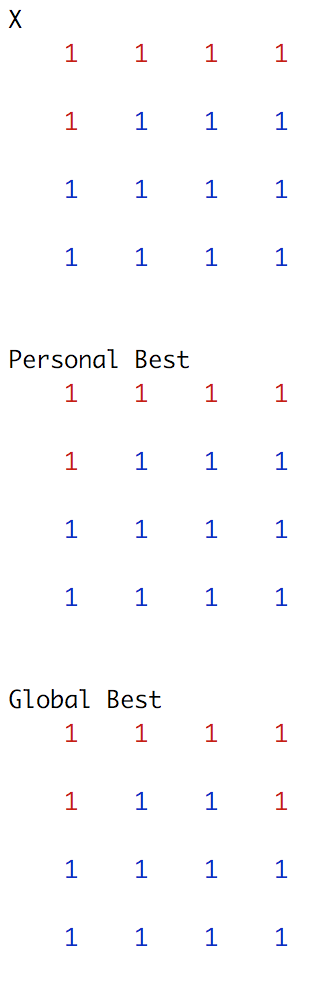
\includegraphics[width=3cm]{pso1.png}
    \centering
    \caption{Example PSO particle, personal best, and global best}
        \label{fig:pso_1}
\end{figure}
\begin{figure}[h!]
    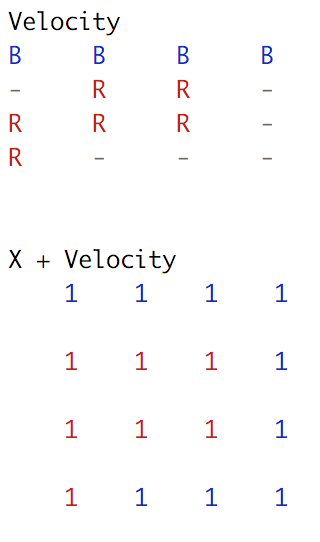
\includegraphics[width=3cm]{pso2.png}
    \centering
    \caption{Example random velocity}
        \label{fig:pso_2}
\end{figure}
\begin{figure}[h!]
    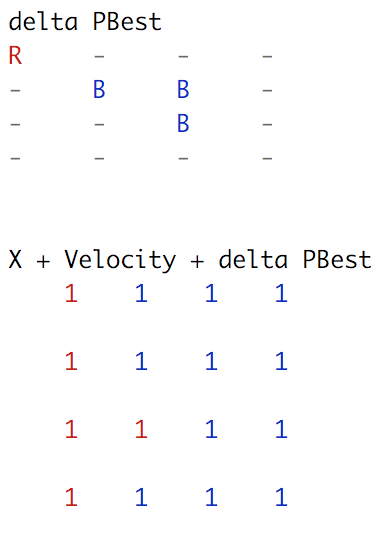
\includegraphics[width=4cm]{pso3.png}
    \centering
    \caption{Swaps to get from (X + Velocity) to Personal Best}
        \label{fig:pso_3}
\end{figure}
\begin{figure}[h!]
    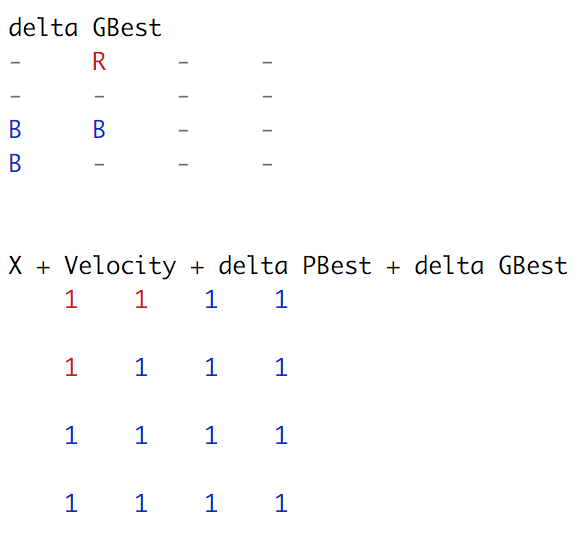
\includegraphics[width=6cm]{pso4.png}
    \centering
    \caption{Swaps to get from (X + Velocity + Pbest) to Global Best}
        \label{fig:pso_4}
\end{figure}

Figure \ref{fig:pso_1} is an example of a particle's current position $X$, it's personal best, and the global best of the swarm. We assume that the values of $w$, $c_1$, $c_2$, $r_1$, and $r_2$ are all $1$ for simplicity in this example. Swaps for the random velocity are capped at 10 swaps, and 4 for the other two velocities for the reasons mentioned in implementation details. This example will only demonstrate one iteration of a single particle for brevity. We show the swaps represented by a velocity as a table of $R$'s and $B$'s as shown in Figure \ref{fig:pso_2}, where the letter represents the district color that the tract in the letter's position should be swapped to.

In order to move the particle to a new position during a single iteration, we first generate a random valid velocity for the particle's current position (limited to a maximum of 10 swaps) and add this velocity to $X$. This new position is shown in Figure \ref{fig:pso_2}.

We then calculate the swaps required from the previous position to the particle's personal best (limited to a maximum of 4 swaps) and add this to the previous position. The resulting position is shown in Figure \ref{fig:pso_3}.

Finally, we calculate the swaps required from the previous position to the swarm's global best (also limited to a maximum of 4 swaps) and add this to the previous position. This will result in the new position of the particle ($X'$) for this iteration as shown in Figure \ref{fig:pso_4}.

\section{Data}
Initially, the proposed solutions are run on experimental data in a grid shape,
known as the Grid Problem. We wanted to apply the solutions on real world data
to observe whether the results are meaningful. Inspired by literature on Tabu
Search implementation, we decided to use data from the state of Iowa to perform
our solution and called it the Iowa Problem. Another motivation to use Iowa was
because of its relatively normal county subdivision without too many
abnormally-shaped counties.

The relevant data for the state of Iowa was fetched in several stages due to
the difficulty of finding consolidated data in one place. From the US census
bureau, we fetched the data for the county shapefiles, which includes
information on the county land/water area, name, shape points and relevant
identifiers such as GeoID. However, in order for the algorithm to work we
also needed information about individual county populations. Fortunately,
there is up-to-date county population data available through Iowa
Demographics\cite{iowa}, which is scraped into a text file. Lastly, the algorithm
also requires data on county adjacencies and the border length between them.
The US census surprisingly provides data on county adjacencies on a nationwide
level\cite{census}, and identifies neighbouring counties by GeoIDs. The border length
can be calculated by combining this information with the relevant shape points
of the neighbouring counties.

Since each county contains a vast collection of shape points to describe its
shape, it becomes a computationally difficult task to find intersecting points
and lines between all counties within the state. Therefore, we applied
approximation on the shape points by taking the absolute top right and bottom
left points, and approximating the shapes into rectangles. Even after the
approximation process we still have an accurate topological mapping of Iowa.
By doing so, we can easily compute the border lengths and create visualizations
to describe the congressional district division of a solution.

\begin{figure}[h!]
    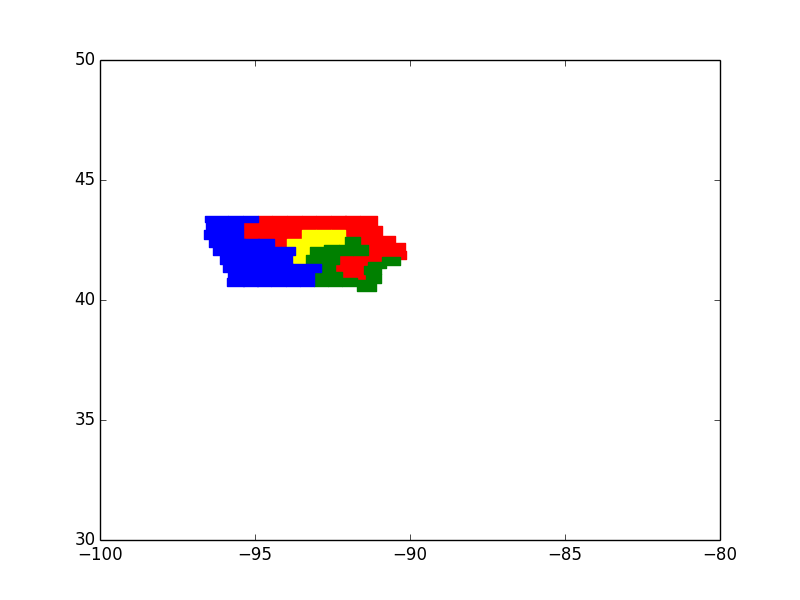
\includegraphics[width=8cm]{iowa.png}
    \centering
    \caption{Visualization of the final congressional district division in the
        state of Iowa using particle swarm solution from one iteration}
    \label{fig:iowa}
\end{figure}

\section{Performance Evaluation}
% Establish a set of evaluation metrics and run some experiments with different
% values of algorithm parameters to quantitatively and qualitatively assess the
% performance of the developed solution using different meta-heuristic
% optimization techniques. Students must identify the pros and cons of each
% technique and assess the quality of work as well as its fit with project
% objectives.

Each algorithm was implemented in Python and tests were run on real data for the state of Iowa from data provided by the U.S. government census data in 2016. For each algorithm we ran a series of tests with 2, 10 and 100 iterations with fixed parameters. The initial parameters for each algorithm were chosen at random within reason. For example, the cooling rate selected for simulated annealing was 0.003. Selecting a faster cooling rate would cause the algorithm to converge to a solution more quickly, which is undesirable.
For each algorithm, the results for each run was recorded. With this data, the minimum, maximum, median and standard deviation were computed for each of the evaluation criteria: compactness, population equality and overall fitness. These criteria were calculated as discussed in Section \ref{sec:proposed_solution} (Proposed Solution). We assumed that all our solutions met the contiguity criteria since this was a hard constraint implemented in each algorithm (i.e. moves or operations were not selected if they resulted in discontinuities). The statistics for each algorithm were then exported to a csv file and graphed, which can be viewed in the tables and figures below.

\subsection{Compactness Results}

\begin{table}[!h]
\centering
\caption{Compactness Results for 100 Iterations on Iowa}
\label{tab:comp_100iter}
\begin{tabular}{l|llll}
                       & \multicolumn{4}{l}{\textbf{Compactness}}                      \\ \hline
\textbf{Algorithm}     & \textbf{min} & \textbf{max} & \textbf{median} & \textbf{stdev} \\ \hline
\textbf{SA}            & 19.255       & 587.016      & 495.146         & 244.594       \\
\textbf{PSO}           & 57.213       & 229.580      & 109.956         & 33.041         \\
\textbf{Hill Climbing} & 52.983       & 264.8        & 122.061         & 41.088         \\
\textbf{Tabu Search}   & 66.946       & 257.239      & 127.855         & 39.242
\end{tabular}
\end{table}

\begin{figure}[h!]
    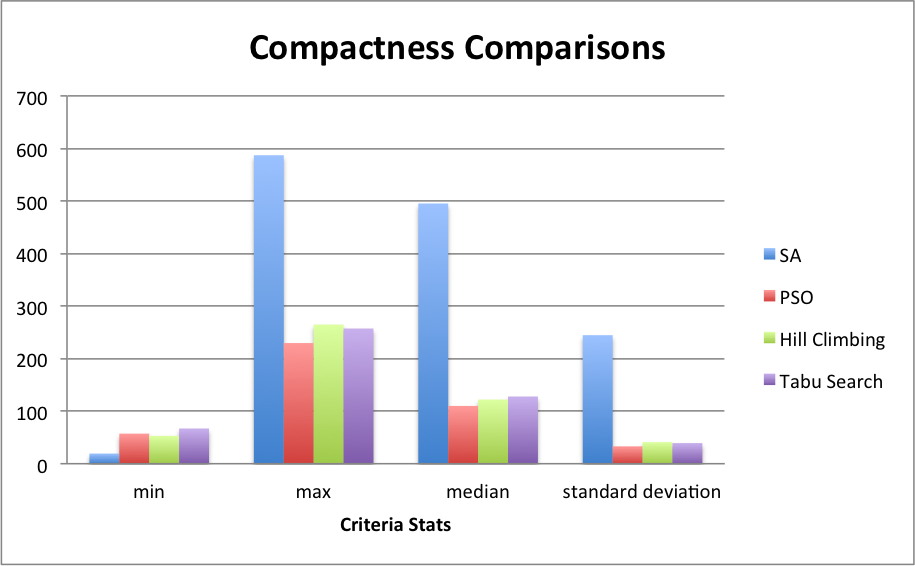
\includegraphics[width=8cm]{images/compactness_graph.png}
    \centering
    \caption{Compactness Results for 100 Iterations on Iowa}
    \label{fig:compactness_results}
\end{figure}

Since our results show the values of cost functions, the lower the value, the better the solution is. Based on the numbers in Table \ref{tab:comp_100iter} as well as Figure \ref{fig:compactness_results}, it is evident that simulated annealing had the most unfavourable compactness results by a significant amount. The other 3 algorithms had similar performance in regards to compactness, but based on our results, PSO generally performed the best, followed by hill climbing and then tabu search.

\subsection{Population Equality Results}

\begin{table}[!h]
\centering
\caption{Population Equality Results for 100 Iterations on Iowa}
\label{tab:pop_100iter}
\begin{tabular}{l|llll}
                       & \multicolumn{4}{l}{\textbf{Population Equality}}             \\ \hline
\textbf{Algorithm}     & \textbf{min} & \textbf{max} & \textbf{median} & \textbf{stdev} \\ \hline
\textbf{SA}            & 1841655      & 4648349.5    & 3098654         & 787073.096         \\
\textbf{PSO}           & 2463         & 94699        & 32829.25        & 15648.72           \\
\textbf{Hill Climbing} & 1749         & 218283       & 9859.75         & 28231.930        \\
\textbf{Tabu Search}   & 36195.5      & 9319.25         & 5647.456       & 5315.779
\end{tabular}
\end{table}

Since the simulated annealing solution had significantly poorer values for population equality as seen in Table \ref{tab:pop_100iter}, they have been excluded in the corresponding graph representation below to better visualize the other algorithm results.

\begin{figure}[h!]
    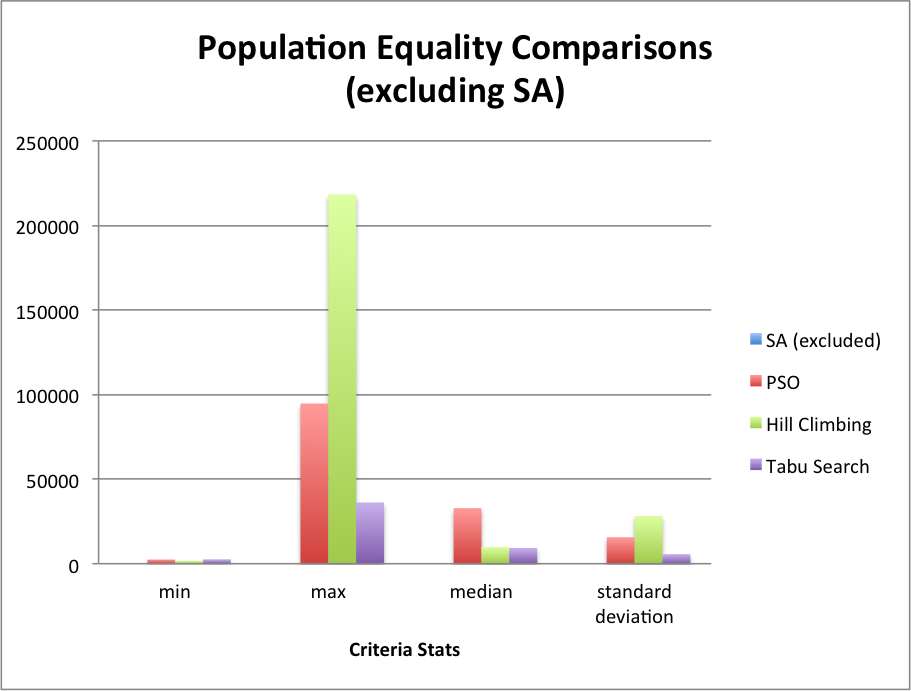
\includegraphics[width=8cm]{images/pop_equality_graph.png}
    \centering
    \caption{Population Equality Results for 100 Iterations on Iowa (excluding SA)}
    \label{fig:pop_results}
\end{figure}

Looking at Figure \ref{fig:pop_results}, we could deduce that hill climbing, although did relatively well in average cases based on the median value, did significantly poorer in certain edge cases as seen from the maximum value. This is most likely as a result of being stuck at a local minima. Looking at the median values, PSO did the most poorly on average, while hill climbing did quite a bit better, and tabu search performed the best. Overall, tabu search had the best (lowest) average population equality cost value, the least deviation, and the smallest maximum cost value. Thus, we can conclude from our results that tabu search performed the best in terms of population equality.

\subsection{Overall Fitness Results}

\begin{table}[!h]
\centering
\caption{Overall Fitness Results for 100 Iterations on Iowa}
\label{tab:fitness_100iter}
\begin{tabular}{l|llll}
                       & \multicolumn{4}{l}{\textbf{Fitness}}                          \\ \hline
\textbf{Algorithm}     & \textbf{min} & \textbf{max} & \textbf{median} & \textbf{stdev} \\ \hline
\textbf{SA}            & 3683810.325  & 9296718.255  & 6197845.196     & 1573915.1    \\
\textbf{PSO}           & 5082.820     & 189513.077   & 65748.985       & 31296.346      \\
\textbf{Hill Climbing} & 3644.275     & 436675.159   & 19839.867       & 56463.519      \\
\textbf{Tabu Search}   & 5315.779     & 72478.096    & 18799.833       & 11289.642
\end{tabular}
\end{table}

Looking at the values in Table \ref{tab:fitness_100iter}, it is evident that simulated annealing performed significantly worse in comparison to the other 3 algorithms, so it has again been excluded in this correspondin graph representation below for better visualization of the other algorithm results.

\begin{figure}[h!]
    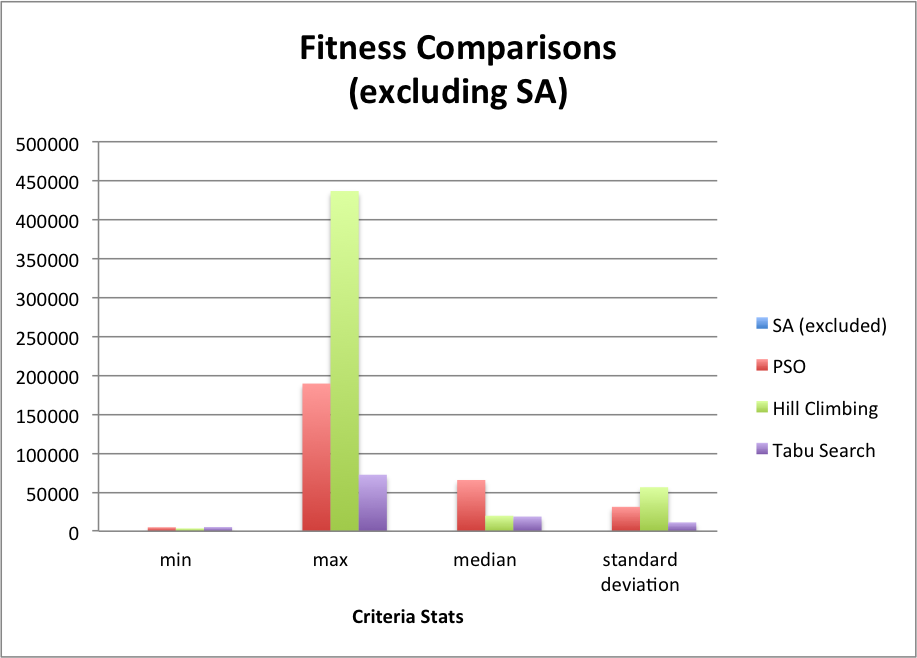
\includegraphics[width=8cm]{images/fitness_graph.png}
    \centering
    \caption{Overall Fitness Results for 100 Iterations on Iowa (excluding SA)}
    \label{fig:fitness_results}
\end{figure}

Figure \ref{fig:fitness_results} shows the results for the overall fitness costs for the algorithms we tested, excluding simulated annealing. The conclusions that can be made are similar to that of the results for population equality. Hill Climbing appeared to work well on average cases, but did significantly poorly in certain edge cases. PSO performed the worst on average, looking at the median values. Tabu Search again performed the best on average cases (it has the lowest median value), had the lowest maximum cost, and the lowest deviation. Based on these results, it can be concluded that for the Iowa state dataset of 2016, tabu search would give the best performance for the Political Districting problem.

\section{Conclusions \& Recommendations}
% Summarize the conclusion and future improvement. Explain how did you solve the
% problem, what problems were met? what did the results show? And how to refine
% the proposed solution? You may organize ideas using lists or numbered points,
% if appropriate, but avoid making your report into a check-list or a series of
% encrypted notes
Our results show that tabu search provides solutions that have the best overall fitness (the least cost) in comparison to the other algorithms we tested. This means that when the tabu search algorithm is run on the data set, it produces solutions that are generally more compact and equal in population than what hill climbing, simulated annealing and particle swarm optimization would produce. Looking at the compactness results from each algorithm, we observe that on average, particle swarm optimization provides better solutions compared to hill climbing, tabu search. Meanwhile, simulated annealing produces large fitness values which are not ideal compared to the other algorithms. Comparing the population equality results we see that simulated annealing again does significantly worse compared to the other algorithms and tabu search did relatively well.

As a result of our experiments and observations of results, it is recommended that further research and parameter tuning effort should be put towards the tabu search algorithm. Tabu search performed the best on average and relatively well when considering each evaluation criteria for political districting. A second recommendation would also be to further research particle swarm optimization methods applied to the political districting problem. Particle swarm optimization performed the second best after observing the results of the overall fitness function.

Given more time, we would have further tuned the parameters for each algorithm. Doing so would allow us to compare the optimal solutions that each algorithm produces. This would give us more accurate insights into which algorithm produces the best results based on the criteria. Running a large number of iterations for certain algorithms was very costly in time and limited us to run at most 100 iterations for each algorithm. In the previous papers we found while researching, we found that the number of iterations done in the different experiments varied from 30 iterations\cite{local-search-2} to 20,000 iterations\cite{geometric-ga}. To justify a reasonable accuracy with 100 iterations, we compared the results between running 10 and 100 iterations, and confirmed that the results were relatively similar.


\begin{thebibliography}{1}
% Every report needs references; in fact, your failure to consult
% references for guidance may be considered negligence. On the other
% hand, when you include sentences, photos, drawings or figures from
% other sources in your report, the complete reference must be cited.
% Failure to do so is plagiarism, an academic infraction with serious
% consequences.

\bibitem{tsp-pso}
    Kang-Ping~Wang et al. Particle Swarm Optimization for Travelling Salesman
        Problem, 2003

\bibitem{voronoi}
    Federica~Ricca et al. Weighted Voronoi region algorithms for political
        districting, 2008

\bibitem{local-search}
    Burcin~Bozkaya et al.  A tabu search heuristic and adaptive memory procedure
        for political districting, 2003

\bibitem{geometric-ga}
    Castelli~Henriques~Vanneschi, A geometric semantic genetic programming system for the electoral redistricting problem, 2014

\bibitem{local-search-2}
    Federica~Ricca et al., Local Search Algorithms for Political Districting, 2007

\bibitem{initial}
    Vickrey, W.: On the prevention of gerrymandering, 1961

\bibitem{census}
    G. Branch. County Adjacency File - Geography - U.S. Census Bureau, 2016

\bibitem{iowa}
    Iowa Demographics. Iowa Counties by Population, 2016

\bibitem{redistricting}
    Levitt, Justin. What is Redistricting? All About Redistricting, 2017.

\bibitem{legislature}
    Redistricting Commissions: State Legislative Plans. National Conference of State Legislature, 2015.

\bibitem{gerry}
    Understanding Congressional Gerrymandering: 'It's Moneyball Applied To Politics'. NPR, 2016.

\end{thebibliography}
\end{document}
